%--------------------------------------------------------------------
%\chapter{Example Section}
%--------------------------------------------------------------------

%%% Local Variables: 
%%% mode: latex
%%% TeX-master: "../D1-2"
%%% End: 

%\subsection*{Geographical Data and Social Media}

Nowadays, the means of public transportation become equipped with physical sensors like GPS sensors or light barriers. Those sensors are used to keep track of the current vehicle position or to estimate the number of passengers. But those sensors do not detect, for instance, emergencies, accidents or the passengers' opinions on bus lines. To overcame these limitations, another kind of sensors is required.

In the last decade, many social networks or micro-blogging services like Twitter\texttrademark arose. They are frequently used by humans to publish their opinions, observations, etc. which then can be requested by a web API. Therefore, the users of those services can be seen as social sensors. The increasing number of mobile phones leads to a situation in which more and more passengers become social sensors by publishing statements about crowded buses or rioting passengers.

The evaluation of the social sensor data requires that the bus or train can be identified to which a message is related. This task is simplified by the fact that most mobile phones have integrated GPS sensors. They measure the current geographical position, which is added to the published message together with a timestamp. This position information can be used to identify the nearest train or bus. A more detailed description of this matching problem  will be given in the next section.

The amount of data produced by the different types of sensors can exceed the processing capabilities of a single computer. Therefore, a distributed approach is required, which will be explained in section \ref{sec:approach}. Finally, the results of an experiment with the current implementation are presented in section \ref{sec:experiment}.

\subsection{Problem of Matching Physical and Social Sensor Data}\label{sec:problem}

In order to find the bus or train a message is related to, the data measured by the physical sensors have to be processed first. In this context, the relevant data consists of the longitude and latitude measured by the GPS sensors of the vehicles. Before transmitting these data, they have to be extended by the unique id of the current vehicle and a timestamp to keep track of the chronological order. The set of all possible position is defined as $Pos$ in equation (\ref{eqn:Pos}).

\vspace*{-2\baselineskip}
\begin{eqnarray}
 Pos & := & V_{id} \times T \times \mathbb{R} \times \mathbb{R}\label{eqn:Pos}
\end{eqnarray}

The relevant data of the social sensors are the messages published by the passengers. Each message contains a timestamp, i.e., the publishing time and the GPS position of the mobile phone from which the message was sent. The set of all possible messages $Mes$ is defined in equation (\ref{eqn:Mes}) where $C$ is the set of all possible message contents.

\vspace*{-2\baselineskip}
\begin{eqnarray}
 Mes & := & T \times \mathbb{R} \times \mathbb{R} \times C\label{eqn:Mes}
\end{eqnarray}

The data of the different sensors are transmitted as a not necessarily finite stream of data as defined in the equations (\ref{eqn:posStream}) and (\ref{eqn:mesStream}).

\vspace*{-2\baselineskip}
\begin{eqnarray}
 posStream: &  & \mathbb{N} \rightarrow Pos\label{eqn:posStream}\\
 mesStream: &  & \mathbb{N} \rightarrow Mes\label{eqn:mesStream}
\end{eqnarray}

The range of $posStream$, i.e., the set of vehicle position received by the data stream $posStream$ are the trajectories of the different vehicles. A trajectory is defined in equation (\ref{eqn:traj}) as a discrete function mapping some point in time to a geographical position.

\vspace*{-2\baselineskip}
\begin{eqnarray}
 traj: & & T \mapsto \mathbb{R} \times \mathbb{R}\label{eqn:traj}
\end{eqnarray}

But this definition is not adequate because the timestamps of messages may vary from the timestamps contained in the position data of the vehicles. Therefore, a continuous trajectory function $\widehat{tray}$ is required. This is reached by, for instance, a linear interpolation of $tray$.

Equation (\ref{eqn:allTraj}) shows the function $allTraj$ which maps the unique identifier of a vehicle on its corresponding continuous trajectory.

\vspace*{-2\baselineskip}
\begin{eqnarray}
 allTraj: & & V_{id} \mapsto (T \mapsto \mathbb{R} \times \mathbb{R})\label{eqn:allTraj}
\end{eqnarray}

In order to relate a message $m$ to a bus or train, the vehicle must be determined which has the smallest euclidean distance $dist$ to the position of the sender at the point in time when $m$ was sent. Furthermore, a vehicle has a maximum length $maxDist$ and all vehicles with a greater distance from $m$ can be ignored. Thus, each message can be seen as a range nearest-neighbour query $rnn$ as defined in equation (\ref{eqn:rnn}).

\vspace*{-2\baselineskip}
\begin{eqnarray}
 &&rnn: Mes \rightarrow Pos \cup \{\texttt{null}\} \textrm{ with}\label{eqn:rnn}\\
 &&rnn((t,lon_m,lat_m,cont)):= (vId,t,lon_v,lat_v)\nonumber\\
 &&\hspace*{1cm}\textrm{if } allTraj(vId)(t)=(lon_v,lat_v) \wedge dist((lon_m,lat_m),(lon_v,lat_v))\leq maxDist \wedge \nonumber\\
 &&\hspace*{1cm}\not\exists vId' \in V_{id}: dist((lon_m,lat_m),allTraj(vId')(t))< dist((lon_m,lat_m),allTraj(vId)(t))\nonumber\\
 &&rnn((t,lon_m,lat_m,cont)):= \texttt{null}\nonumber\\
 &&\hspace*{1cm}\textrm{otherwise}\nonumber
\end{eqnarray}

Putting it all together, the problem of finding the nearest vehicle for each message is defined as followed:

{
\definecolor{mygray}{gray}{.75}
\fbox{\colorbox{mygray}{\parbox{\columnwidth}{
\textbf{Problem} Finding range nearest vehicle for each message\\
\textbf{Input:} $posStream$, $mesStream$, $maxDist$\\
\textbf{Output:} $rnnStream: \mathbb{N} \rightarrow Mes \times Pos \bullet rnnStream(i):=(mesStream(i),rnn(mesStream(i)))$
}}}
}

An implementation which solves this problem has to deal with the fact, that the data received by different sensors are not equally delayed. For instance, the data measured from physical sensors may be faster transmitted then messages received from social networks.

Another difficulty is, that the amount of data received by the different input streams may exceed the processing capabilities of a single computer. One solution for this problem would be to discard incoming data if the load of the single machine would be to high. This could lead to the loss of valuable data. In order to avoid this, a distributed approach is required which scales horizontally.

Some approaches like PLACE* \cite{Xiong2007PAD} distribute the incoming data according to a static mapping of computers on geographical regions. The disadvantage of this static mapping can be seen, for instance, if there exists a sport stadium in some region. If a sport event takes place, then there are many vehicles and passengers producing a huge amount of data. Therefore, the corresponding computer can only deal with a relatively small region. But if not event takes places, this computer does nearly have no work. In order to improve this, the mapping has to be dynamic, i.e., a dynamic load balancing is required.

\subsection{Distributed Geo-Matching Approach}\label{sec:approach}

The schema of an intuitive stream-processing system which solves the problem described above can be seen in figure \ref{subfig:localRtree}. It consists of a single component ($C$) which receives the incoming data streams of vehicle positions and messages. It caches the current positions and processes the range nearest-neighbour queries initiated by the received messages. The answers are transmitted via the outgoing data stream $rnnStream$.

In order to answer range nearest-neighbour queries, $C$ has to cache the current position of all vehicles. The problem of the delayed sensor data requires the caching of more vehicle positions than just the latest. Thus, a sliding window approach is implemented with a window size exceeding all regular delay times. This is realized by deleting all vehicle positions outside the window whenever a new position with a timestamp later then the timestamp of the latest cached position is received.

The data structure used as cache should answer range nearest-neighbour queries efficiently. In spatio-temporal databases R*-trees \cite{Beckmann1990TRA} are used for this purpose. Similar to a B-tree, the inserted elements are stored only in the leafs. Each node except the root has a minimal and a maximal number of children or elements. If an insertion is performed on a node already containing the maximal number of elements, then it is split and the resulting inner node is inserted in the parent node. In contrast to B-trees, each node of an R*-tree represents the minimal bounding rectangle (MBR) of all elements contained in its subtree as illustrated in figure \ref{fig:Rtree}. The presented tree consists of a root node (dark gray), seven leafs (light gray) and several vehicle positions (black squares).

\begin{figure}[htbp]
\centering
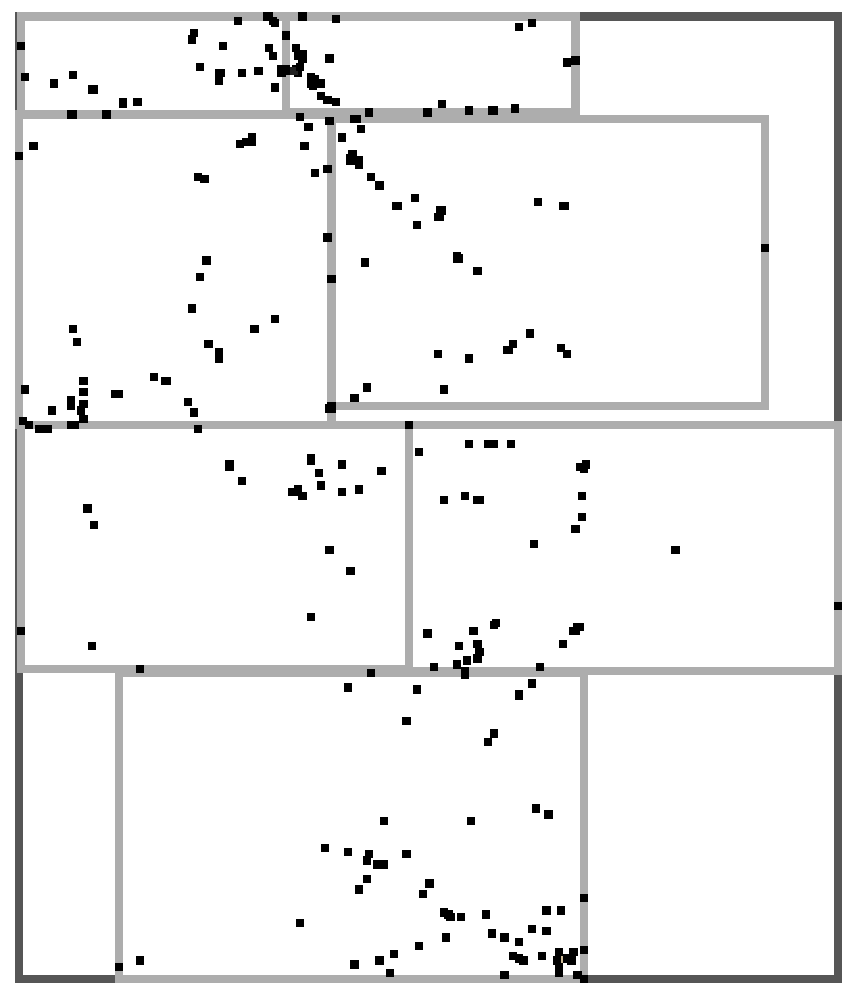
\includegraphics[scale=0.3,angle=90]{img/dgm/rTree.pdf}
\caption{An examplary R*-tree}\label{fig:Rtree}
\end{figure}

During the processing of a range nearest-neighbour query, only the children of a node are visited whose MBR intersects with the queried range. Thus, the performance of the query processing depends on the number of subtrees to be traversed. In order to reduce this number, the MBRs of the child nodes should be disjoint. As shown in \cite{Beckmann1990TRA} the algorithms used for insertion and deletion are designed to ensure a minimal overlap of MBRs. Another advantage is, that the MBRs are dynamically adjusted according to the currently contained elements.

\begin{figure}[htbp]
\centering
\subfigure[A system with a single cache]{
\label{subfig:localRtree}
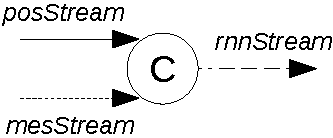
\includegraphics[scale=0.6]{img/dgm/SingleCache.pdf} 
}
\subfigure[A system with several caches]{
\label{subfig:rootRtree}
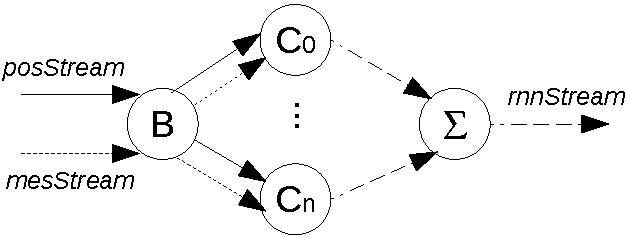
\includegraphics[scale=0.6]{img/dgm/MultiCache.pdf} 
}
\subfigure[A distributed R*-tree]{
\label{subfig:distributedRtree}
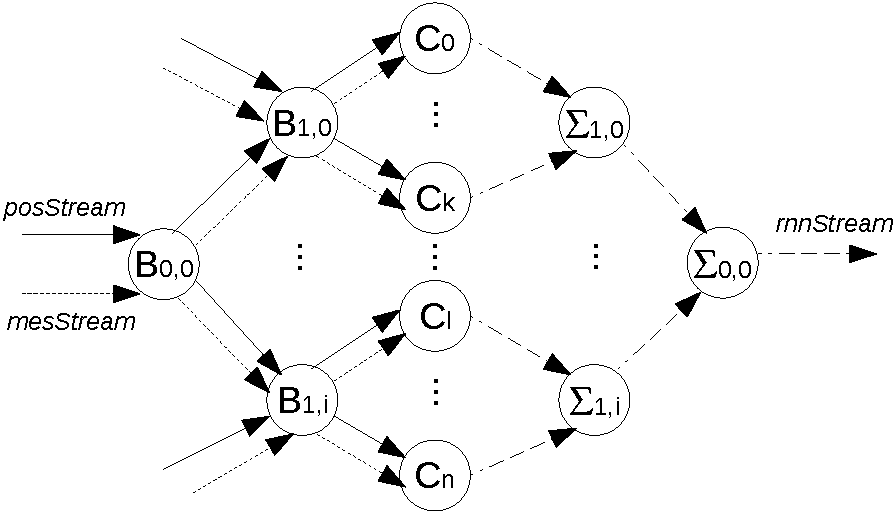
\includegraphics[scale=0.6]{img/dgm/DistributedTree.pdf} 
}
\caption{Distributing a geo-matching system}\label{fig:DistributedRtree}
\end{figure}

The problem of the system shown in figure \ref{subfig:localRtree} is that its processing capabilities are quite limited. Therefore, a distributed approach is required which spreads the load on several computers. Figure \ref{subfig:rootRtree} shows such a system. It consists of several caches $C_0$ to $C_n$ each of them owning an own R*-tree for caching current vehicle positions and responding to queries.

Furthermore, this system consists of balancer component $B$. It receives the incoming streams of vehicle positions and messages and decides to which of the different caches each single datum is sent. Similar to the root of an R*-tree, it keeps track of the MBRs of the different caches. A new vehicle position is basically sent to the cache with the nearest MBR. If $B$ receives a new message, it is only forwarded to the caches whose MBR intersects with the queried range. In the best case this is only one cache. But it could be several caches as well. Thus a special combiner component ($\Sigma$) is required which receives the nearest vehicle of each cache involved inte the query processing and returns the overall nearest neighbour.

A further responsibility of $B$ is the load balancing, i.e., the number of cached vehicle positions and queries in progress should be similar for all caches. Therefore, $B$ counts the number of vehicle positions and messages forwarded to the different caches. The load balancing is done by distributing the received vehicle positions according to special target ranges for the different caches. In the case of a balances system, these regions are equal to the MBRs. But if the load of a cache $C_i$ exceeds the load of a cache $C_j$ with a neighboured MBR, than the target range of $C_i$ is reduced and the range of $C_j$ increased. During the progress of the sliding window the MBRs of the caches will approach their target ranges.

In regular intervals, $B$ sends special requests to all caches to send the information about their current loads and MBRs back (not shown in figure \ref{subfig:rootRtree}). If $B$ receives the responses of all caches, it updates its calculated values. These update requests are performed asynchronously, i.e., the distribution of the incoming data is not blocked. This leads to a situation that the information received by the caches are not up to date any more. Therefore, $B$ caches all forwarding decisions from the time the updated request is sent until all caches have responded. Then these decisions are applied on the received load information and MBRs.

The disadvantage of this system is, that the single balancer component $B$ and combiner component $\Sigma$ can become bottlenecks. A future solution could be found when thinking of $B$ as the root of distributed R*-tree whose children are the trees stored in the different caches. If it is close to its processing limits, it creates child balancer components which are responsible for subregions of the overall MBR. Each of the children gets an input stream for all the data of its MBR. Data for regions which are not covered by the children are still received by the root. Whenever a balancer component is split the combiner components are split analogously. Such a system is illustrated in figure \ref{subfig:distributedRtree}.

\subsection{Experiment}\label{sec:experiment}
